\documentclass[11pt]{article}
 
\usepackage[top=0.75in, bottom=1.25in, left=1in, right=1in]{geometry} 
\usepackage{amsmath,amsthm,amssymb} %this is THE math package
\usepackage{mathtools}
\usepackage{tikz}
\usepackage{graphicx}
\usepackage{fancybox}
\usepackage{hyperref}
\usepackage{varwidth}
\usepackage{mdframed}
\usepackage{mathrsfs}
\usepackage[most]{tcolorbox}
%------------------------
%Fonts I use, uncomment if you like to use them.
%The first is the general font, and the second a math font
\usepackage{mathpazo}
\usepackage{eulervm}
%------------------------
%This is so that we have standard fonts for the double-stroked symbols
%for reals, naturals etc. regardless of what font you use.
%Don't comment
\AtBeginDocument{
  \DeclareSymbolFont{AMSb}{U}{msb}{m}{n}
  \DeclareSymbolFontAlphabet{\mathbb}{AMSb}}
%------------------------
\usepackage{graphicx}
\graphicspath{ {./images/} }
%----------------------------------------------
%User-defined environments
%Commented because we're not using them in this document
%The only uncommented ones are the Problem and Solution environment

% \newenvironment{theorem}[2][Theorem]{\begin{trivlist}
% \item[\hskip \labelsep {\bfseries #1}\hskip \labelsep {\bfseries #2.}]}{\end{trivlist}}
% \newenvironment{lemma}[2][Lemma]{\begin{trivlist}
% \item[\hskip \labelsep {\bfseries #1}\hskip \labelsep {\bfseries #2.}]}{\end{trivlist}}
% \newenvironment{exercise}[2][Exercise]{\begin{trivlist}
% \item[\hskip \labelsep {\bfseries #1}\hskip \labelsep {\bfseries #2.}]}{\end{trivlist}}
% \newenvironment{question}[2][Question]{\begin{trivlist}
% \item[\hskip \labelsep {\bfseries #1}\hskip \labelsep {\bfseries #2.}]}{\end{trivlist}}
% \newenvironment{corollary}[2][Corollary]{\begin{trivlist}
% \item[\hskip \labelsep {\bfseries #1}\hskip \labelsep {\bfseries #2.}]}{\end{trivlist}}
\newenvironment{problem}[2][Problem\!]{\begin{trivlist}
\item[\hskip \labelsep {\bfseries #1}\hskip \labelsep {\bfseries #2}]}{\end{trivlist}}
%\newenvironment{sub-problem}[2][]{\begin{trivlist}
%\item[\hskip \labelsep {\bfseries #1}\hskip \labelsep {\bfseries #2}]}{\end{trivlist}}
\newenvironment{solution}{\begin{proof}[\textbf{\textit{Solution}}] }{\end{proof}}
%----------------------------------------------

%----------------------------
%User-defined notations
\newcommand{\zz}{\mathbb Z}   %blackboard bold Z
\newcommand{\qq}{\mathbb Q}   %blackboard bold Q
\newcommand{\ff}{\mathbb F}   %blackboard bold F
\newcommand{\rr}{\mathbb R}   %blackboard bold R
\newcommand{\nn}{\mathbb N}   %blackboard bold N
\newcommand{\cc}{\mathbb C}   %blackboard bold C
\newcommand{\af}{\mathbb A}   %blackboard bold A
\newcommand{\pp}{\mathbb P}   %blackboard bold P
\newcommand{\id}{\operatorname{id}} %for identity map
\newcommand{\im}{\operatorname{im}} %for image of a function
\newcommand{\dom}{\operatorname{dom}} %for domain of a function
\newcommand{\cat}[1]{\mathscr{#1}}   %calligraphic category
\newcommand{\abs}[1]{\left\lvert#1\right\rvert} %for absolute value
\newcommand{\norm}[1]{\left\lVert#1\right\rVert} %for norm
\newcommand{\modar}[1]{\text{ mod }{#1}} %for modular arithmetic
\newcommand{\set}[1]{\left\{#1\right\}} %for set
\newcommand{\setp}[2]{\left\{#1\ \middle|\ #2\right\}} %for set with a property
\newcommand{\card}[1]{\#\,{#1}} %for cardinality of a set
\newcommand\m[1]{\begin{pmatrix}#1\end{pmatrix}} 

%Re-defined notations
\renewcommand{\epsilon}{\varepsilon}
\renewcommand{\phi}{\varphi}
\renewcommand{\emptyset}{\varnothing}
\renewcommand{\geq}{\geqslant}
\renewcommand{\leq}{\leqslant}
\renewcommand{\Re}{\operatorname{Re}}
\renewcommand{\Im}{\operatorname{Im}}
%----------------------------

\allowdisplaybreaks
 
 
\begin{document}
 
\title{12/06 Submission}
\author{Kevin Guillen\\[0.5em]
MATH 101  | Math 200 | Fall 2021}
\date{} 
\maketitle

%Use \[...\] instead of $$...$$

\begin{tcolorbox}
    \begin{problem} {IC | 12-03 | PP 40}
        A right circular cone has base of radius 1 and height 3. A cube is inscribed in the cone so that one face of the cube is contained in the base of the cone. What is the side length of the cube?
    \end{problem}
\end{tcolorbox}
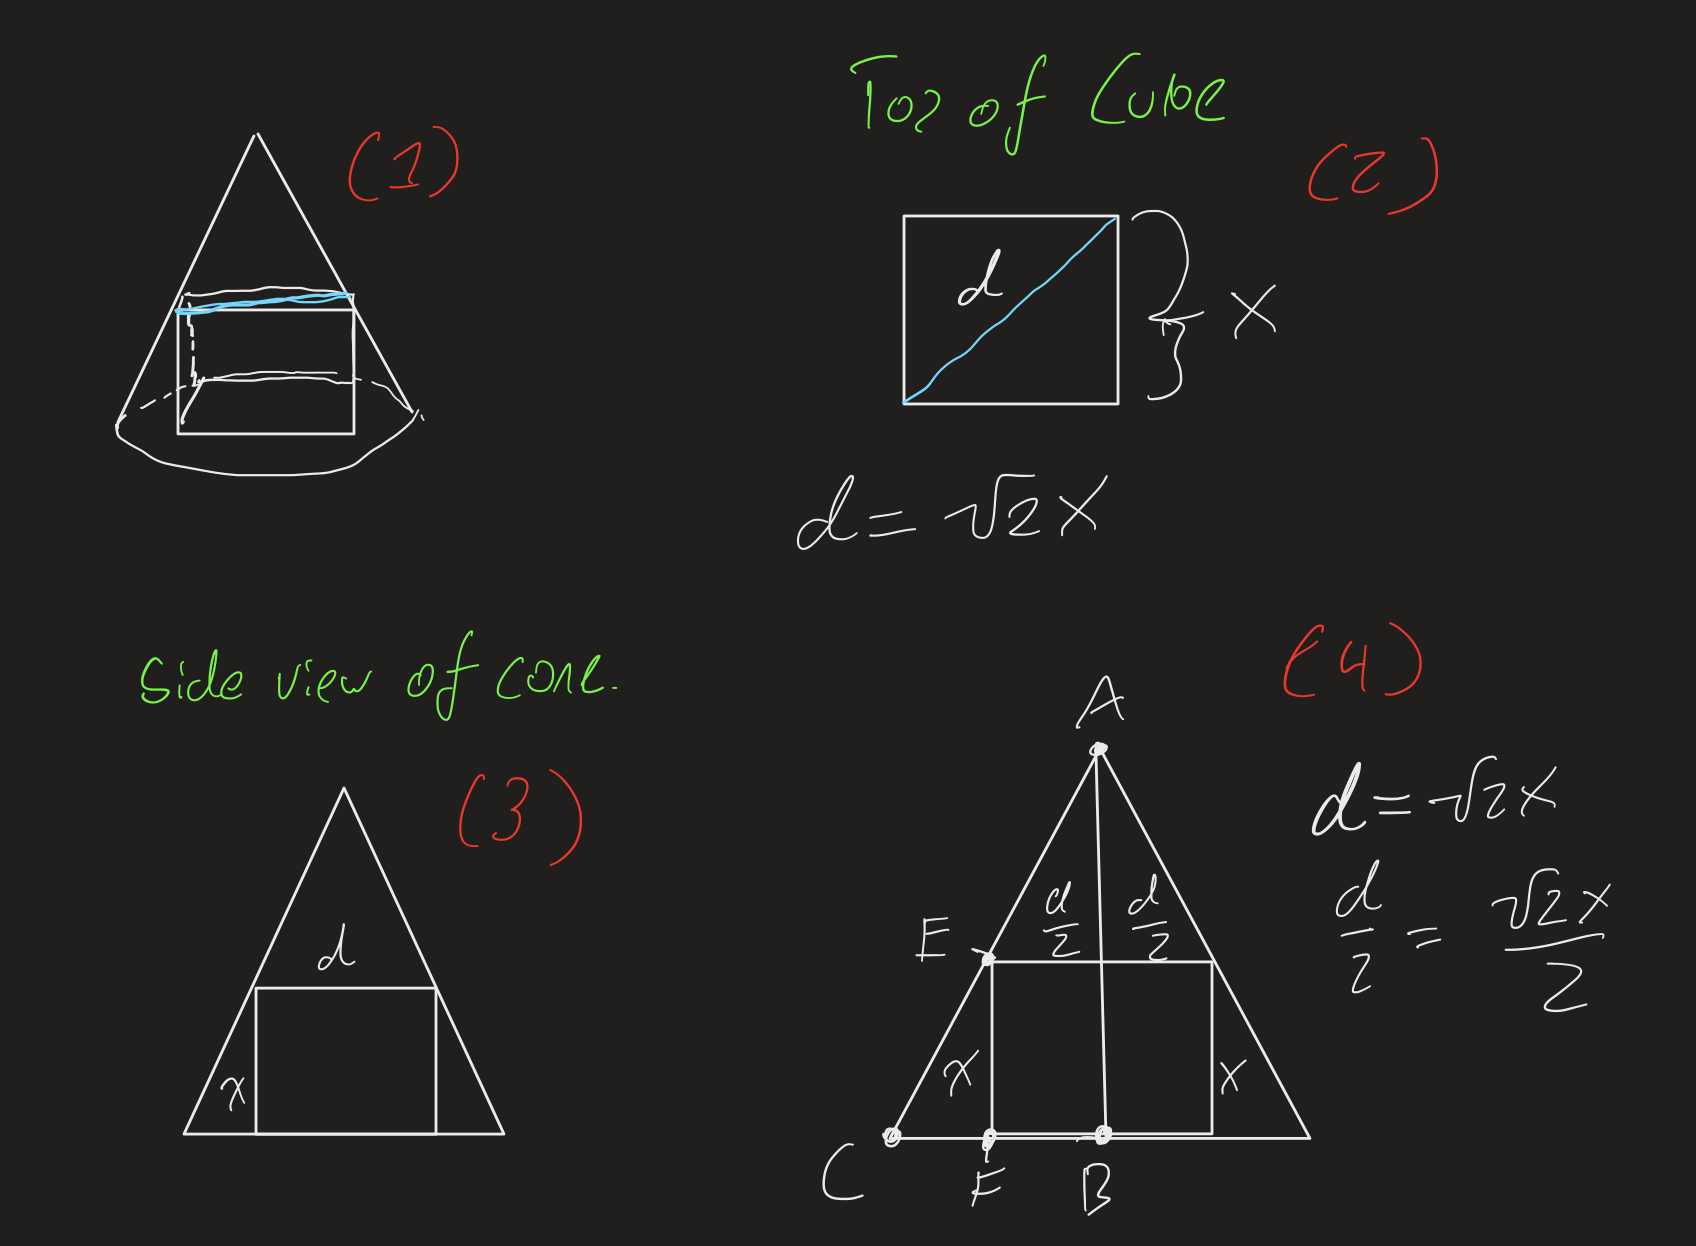
\includegraphics[scale=0.5]{diagram}
\begin{proof}
    Consider the cube inscribed in a cone as in image (1), where the lengths of each side are denoted by $x$, and the diagonal of the top of the cube is denoted by $d$ as seen in (2). We know that $d = \sqrt2 x$. Now consider the side view of the cone such that our view is perpendicular to the top diagonal of the square as seen in (3). We can bisect this triangle along its apex to obtain two more triangles as seen in (4). Each of these new triangles will then have a rectangle of side lengths $x$ and $\frac{d}{2}$. We see that the triangle formed by $ABC$ is similar to $CEF$. This gives us the following equation,
    \begin{align*}
        \frac{1}{3} = \frac{1-\frac{d}{2}}{x} = \frac{1- \frac{\sqrt2 x}{2}}{x}
    \end{align*}
    now let's solve for $x$,
    \begin{align}
        x &= 3 - \frac{3\sqrt2 x}{2}\\
        x + \frac{3\sqrt2 x}{2} &= 3 \\
        x(1 + \frac{3\sqrt 2}{2}) &= 3 \\
        x &= \frac{3}{1 + \frac{3\sqrt2}{2}} \approx 0.9661
    \end{align}
\end{proof}

\begin{tcolorbox}
    \begin{problem} {IC | 12/03 | PP 41.}
        Find the minimum value of $\dfrac{(x+\frac{1}{x})^{6} - (x^{6}+\frac{1}{x^{6}}) -2)}{(x+\frac{1}{x})^{3} + (x^{3} + \frac{1}{x^{3}})}$ for $x > 0$
    \end{problem}
\end{tcolorbox}
\begin{proof}
    First let us manipulate the numerator so that we can substitute $x + \frac{1}{x}$ with $y$.
    \begin{align}
        (x+\frac{1}{x})^{6} - (x^{6} + \frac{1}{x^{6}}) -2 &= (x+ \frac{1}{x})^{6} - (x^{2} + \frac{1}{x^{2}})(x^{4} + \frac{1}{x^{4}} - 1) - 2 \\
        &= (x + \frac{1}{x})^{6} - ((x + \frac{1}{x})^{2}-2)((x^{2} + \frac{1}{x^{2}})^{2} - 3) - 2 \\
        &= (x + \frac{1}{x})^{6} - ((x + \frac{1}{z})^{2} - 2)(((x + \frac{1}{x})^{2} - 2)^{2} -3) - 2 \\
        &= y^{6} - (y^{2} - 2)((y^{2}-2)^{2} - 3) - 2 \\
        &= 
    \end{align}
\end{proof}
\begin{tcolorbox}
  \begin{problem} {IC | 12-03 | PP 42}
    Let $k > 1$ be a positive integer. Show that the equation $x^{2} -y^{2} = k^{3}$
always has integral solutions in $x$ and $y$.
  \end{problem}
\end{tcolorbox}
\begin{proof}
    Consider the following,
    \begin{align*}
        x^{2} + y^{2} &= k^{3} \\
        (x+y)(x-y) &= (k)(k^{2})
    \end{align*}
    this gives us the system of equations,
    \begin{align*}
        (x+y) &= k^{2} \\
        (x-y) &= k.
    \end{align*}
    We know that $k^{2} - k$ and $k^{2} +k $ will yield an even integer for any $k \in \zz$ since squaring a number preserves parity. This lets us set $x = \frac{k^{2} + k}{2}$ and $y = \frac{k^{2} - k}{2}$. We see then,
    \begin{align}
        (x+y)(x-y) &= (\frac{k^{2} + k}{2} + \frac{k^{2} - k}{2})(\frac{k^{2} + k}{2} -\frac{k^{2} - k}{2}) \\
        &= \frac{2k^{2}}{2}\frac{2k}{2} \\
        &= k^{2}k\\
        &= k^{3}
    \end{align}
    meaning $x^{2}-y^{2} = k^{3}$ always has integral solutions in $x$ and $y$.
\end{proof}

\end{document}